\documentclass[paper=a4, fontsize=11pt]{scrartcl}

\usepackage{fancyhdr}
\pagestyle{fancyplain}
\setlength{\headheight}{25pt}
\renewcommand{\headrulewidth}{0pt}
\renewcommand{\footrulewidth}{0pt}
\usepackage{graphicx}
\usepackage{epigraph}
\usepackage{amsmath,amssymb,amsfonts }
\usepackage{lastpage}
\usepackage{algorithm}
\usepackage{algpseudocode}
\usepackage{csquotes}


\newcommand{\Abf}{\ensuremath{\mathbf{A}}}
\newcommand{\bbf}{\ensuremath{\mathbf{b}}}
\newcommand{\cbf}{\ensuremath{\mathbf{c}}}
\newcommand{\abf}{\ensuremath{\mathbf{a}}}
\newcommand{\xbf}{\ensuremath{\mathbf{x}}}
\newcommand{\ybf}{\ensuremath{\mathbf{y}}}
\newcommand{\Rbb}{\ensuremath{\mathbb{R}}}
\newcommand{\Rbf}{\ensuremath{\mathbf{R}}}
\newcommand{\fo}{\ensuremath{f_0}}
\newcommand{\fii}{\ensuremath{f_i}}
\newcommand{\transpose}[1]{#1^\mathsf{T}}
\newcommand{\norm}[1]{\ensuremath{\lVert{#1}\rVert}}


\newtheorem{definition}{Definition}[section]
\newtheorem{theorem}{Theorem}[section]
\newtheorem{lemma}[theorem]{Lemma}
\newtheorem{proposition}[theorem]{Proposition}
\newtheorem{corollary}[theorem]{Corollary}
\newtheorem{observation}[theorem]{Observation}

\newenvironment{proof}[1][Proof]{\begin{trivlist}
\item[\hskip \labelsep {\bfseries #1}]}{\end{trivlist}}
%\newenvironment{definition}[1][Definition]{\begin{trivlist}
%\item[\hskip \labelsep {\bfseries #1}]}{\end{trivlist}}
\newenvironment{example}[1][Example]{\begin{trivlist}
\item[\hskip \labelsep {\bfseries #1}]}{\end{trivlist}}
\newenvironment{remark}[1][Remark]{\begin{trivlist}
\item[\hskip \labelsep {\bfseries #1}]}{\end{trivlist}}

\newcommand{\qed}{\nobreak \ifvmode \relax \else
      \ifdim\lastskip<1.5em \hskip-\lastskip
      \hskip1.5em plus0em minus0.5em \fi \nobreak
      \vrule height0.75em width0.5em depth0.25em\fi}


\newcommand{\lecture}{Homework \#5 Report} %lecture number and date goes here
\newcommand{\lecturedate}{Due: May 23, 2016} %lecture date goeshere
\newcommand{\scribe}{Michael Lam} %student name goes here

\fancyhead[L]{\small Spring 2016}
\fancyhead[R]{\small \lecture}
%\fancyfoot[L]{\small CS 533: Intelligent Agents and Decision Making}
%\fancyfoot[C]{}
\fancyfoot[C]{\thepage\ of \pageref{LastPage}}


\begin{document}


\newcommand{\horrule}[1]{\rule{\linewidth}{#1}} % Create horizontal rule command with 1 argument of height

\title{	
\normalfont \normalsize
\vspace{-30pt}
\textsc{CS 533: Intelligent Agents and Decision Making} \\ [10pt]
\horrule{0.5pt} \\[0.4cm] % Thin top horizontal rule
\LARGE \lecture\\ % The assignment title
\vspace{5pt}
\normalsize \scribe\\
\lecturedate\\
\horrule{2pt} \\[0.5cm] % Thick bottom horizontal rule
}


\date{} % Today's date or a custom date

\maketitle
\vspace{-100pt}
%\epigraph{''Every problem is an optimization problem in disguise.''}{--Anonymous}

\begin{abstract}
This assignment explores policy simulation of a ``parking'' MDP and implements a reinforcemnet learning agent for this environment.
\end{abstract}

\section{Part I}

We designed our MDP as suggested, only we further factorize location $L$ into column $C \in \{A, B\}$ and row $R \in \{1, 2, \ldots, n\}$ where $n$ is the number of parking rows. Therefore our state is a 4-tuple $(C, R, O, P)$, which just makes the location more explicit.

We experimented with two sets of parameters. We made the following assumptions for the first one (``MDP1''), which we will call the ``reasonable driver'':

\begin{itemize}
\item The reward for states without being parked is $-1$ to discourage from driving too much.
\item The reward for parking as a function of being in row $r \in \{2, 3, \ldots, n\}$ (note: not in handicap spot) is $(n-(r-1))/(n-1) \cdot F$, where $F=10$ is an adjustable reward factor. It is more desirable to park nearer to the store.
\item The reward for parking in the handicap spots is $-100$. The assumption here is that the driver really doesn't want to risk a ticket.
\item The reward for parking in an occupied spot, i.e. collision, is $-10000$. Collisions are really, really bad.
\item The reward for the terminal state is $1$. The terminal state also has no transitions so it's the last state.
\item After a DRIVE action, if the next spot is not a handicap spot, the probability that the next spot is occupied by another car is a linear function of the row $r$: $(n-(r-1))/(n-1)$. As the row goes further away from the store, the probability of being occupied is decreased.
\item After a DRIVE action, if the next spot is a handicap spot, the probability that the next spot is occupied by another car is fixed at $0.001$, which is a relatively small probability.
\end{itemize}

The second one (``MDP2''), which we will denote as ``ignorant driver'', is the same as above except for the following:

\begin{itemize}
\item The reward for parking in a handicap spot is $100$. The driver doesn't care about getting a ticket and just wants a spot, especially at the front of the store!
\end{itemize}

This one modification is good enough to test the algorithms and policies. It would make sense that the policies of the reasonable driver and ignorant driver would give different average total rewards. We will test this.

In all the experiments, we set number of rows $n=10$. We set the discount factor $\beta = 0.99$, which is close to $1$ to let the behavior be mainly influenced by the MDP dynamics and reward.

We use policy iteration to get the exact optimal policy, which will be checked against the manual policies specified in Part II and the policy learned by a reinforcement learning agent in Part III.

\section{Part II}

\subsection{Design}

Our custom policy is as follows:

\blockquote{The policy selects DRIVES whenever O is TRUE. When O is FALSE and the current spot is a handicap, the policy selects PARK with probability $p_h$ and otherwise DRIVES with probability $1-p_h$. Otherwise when O is FALSE and the current spot is not a handicap, the policy selects PARK with probability $p$ and otherwise DRIVES with probability $1-p$.}

Essentially, we add another parameter called the handicap parking probability $p_h$. Note that $p_h=0$ means the agent will never park in the handicap spot and $p_h=1$ means the agent will always park in the handicap spot when it is not occupied. We experiment with $p_h=0$ and $p_h=1$ in our experiments.

Besides our custom policy, we can also compute the optimal policy of the MDPs. We use the policy iteration algorithm from the prior assignment to compute the optimal policy. This will be useful to compare against the other policies as well as use in Part III.

\subsection{Results/Experiments/Discussion}

We plot the table of average total reward from simulating the two MDPs on various policies in Table \ref{tab:policies}. The random policy performs the worst, which makes sense since the policy does not handle collisions. The safe random policy (where it always DRIVES on O is TRUE) performs better as it never causes collisions. However, as it still uses randomness to determine whether to park, it can still be better by reasoning the current row and whether it's a handicap spot.

Our custom policy handles the handicap spot with a probability. By setting $p_h=0$, the agent will never park at a handicap spot. By setting $p_h=1$, the agent will always park at a hanicap spot if it is not occupied. For MDP1, we see that $p_h=0$ gives better results than the safe random policy and we see that $p_h=1$ performs poorly. This makes sense since in MDP1, there is negative reward for parking at a handicap spot so avoiding it is an improvement over the safe random policy, but forcing to park at a handicap spot yields very poor results from the penalty of parking in a handicap spot. For MDP2, we see that $p_h=1$ gives better results than the safe random policy and we see that $p_h=0$ gives poorer results than the safe random policy but it is not drastically bad. This makes sense since in MDP2, there is high reward for parking in the handicap spot so forcing to park in the handicap spot is good, while avoiding the handicap spot is still okay but does not yield as high of a reward.

Finally, we see that all of our manual policies perform worse than the optimal policy. This makes sense since none of our manual policies reasoned about the row the agent is in; we can do better. In Part III, we will construct a reinforcement learning agent which will hopefully learn the optimal policy.

\begin{table}
\begin{center}
\captionof{table}{Average Total Reward of Various Policies and MDPs} \label{tab:policies}
\begin{tabular}{ | l |c|c| }
  \hline
  Policy & MDP1 & MDP2\\ \hline
  Random & -3932.09 & -3712.91\\ \hline
  Safe Random & 10.28 & 26.23\\ \hline
  Custom $p_h=0$ & 21.811 & 20.512\\ \hline
  Custom $p_h=1$ & -50.975 & 64.576\\ \hline
  Optimal & 78.484 & 89.06\\ \hline
\end{tabular}
\end{center}
\end{table}

\section{Part III}

\subsection{Design}

We implemented a model-free reinforcement learning agent for the environment using Q-learning. It stores a Q-table of states and actions.

For the explore/exploit policy, we use $\epsilon$-greedy: with $\epsilon$ probability, choose a random action for exploration, otherwise exploit using the current Q-table. We investigate various $\epsilon$ settings in our experiments.

To speed up learning, we use reverse updates. We store the trajectory of a learning trial and do the Q-updates in reverse order. We will also explore different learning rates $\alpha$ in our experiments.

\subsection{Experiments/Results}

We run $N=10,000$ learning trials to perform Q-updates, then run $1,000$ trials without learning to get the average total reward. We repeat this $15$ times, which we denote as the number of epochs (epoch 0 is the result after running the first $N=10,000$ learning trials and $1,000$ trials without learning). We experimented by varying two sets of parameters: learning rate $\alpha$ and explore/exploit parameter $\epsilon$.

We experimented with various fixed $\epsilon$ parameters: $\epsilon=0.1,0.25,0.5,0.75$. The graphs are plotted for MDP1 and MDP2 in Figures \ref{fig:mdp1_epsilon} and \ref{fig:mdp2_epsilon}. We also experimented with various fixed learning rate $\alpha$ parameters: $\alpha=0.001, 0.01,0.1,1.0$. The graphs are plotted for MDP1 and MDP2 in Figures \ref{fig:mdp1_alpha} and \ref{fig:mdp2_alpha}.

\begin{figure}
\centering
	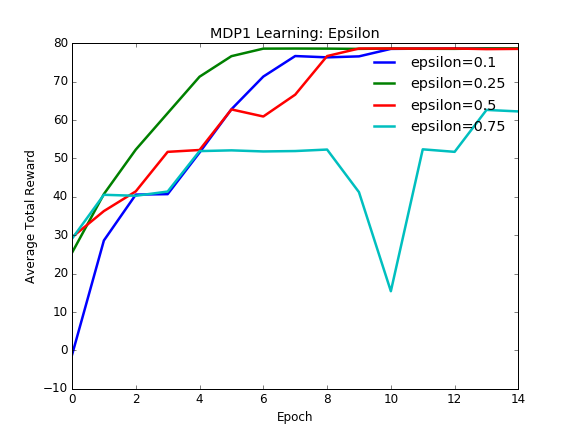
\includegraphics[width=.8\linewidth]{mdp1_epsilon_plot.png}
\caption{Plot of average total reward as a function of epochs for different $\epsilon$ values using MDP1 and fixing learning rate $\alpha=0.01$.}
\label{fig:mdp1_epsilon}
\end{figure}

\begin{figure}
\centering
	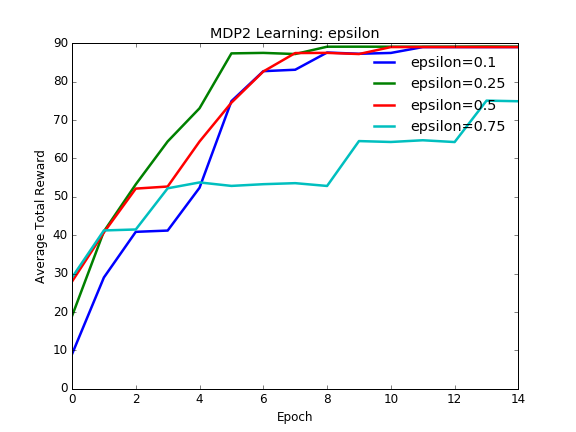
\includegraphics[width=.8\linewidth]{mdp2_epsilon_plot.png}
\caption{Plot of average total reward as a function of epochs for different $\epsilon$ values using MDP2 and fixing learning rate $\alpha=0.01$.}
\label{fig:mdp2_epsilon}
\end{figure}

\begin{figure}
\centering
	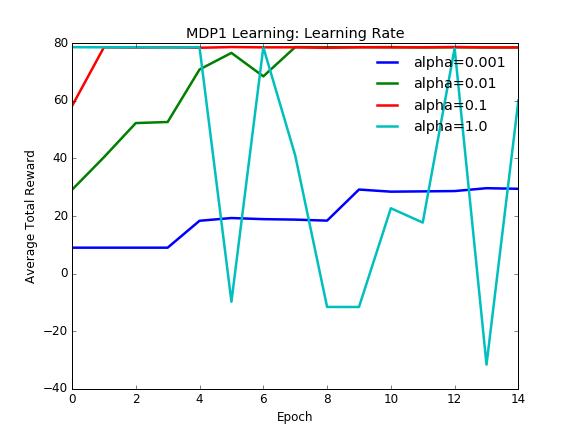
\includegraphics[width=.8\linewidth]{mdp1_alpha_plot.png}
\caption{Plot of average total reward as a function of epochs for different learning rate $\alpha$ values using MDP1 and fixing $\epsilon=0.1$.}
\label{fig:mdp1_alpha}
\end{figure}

\begin{figure}
\centering
	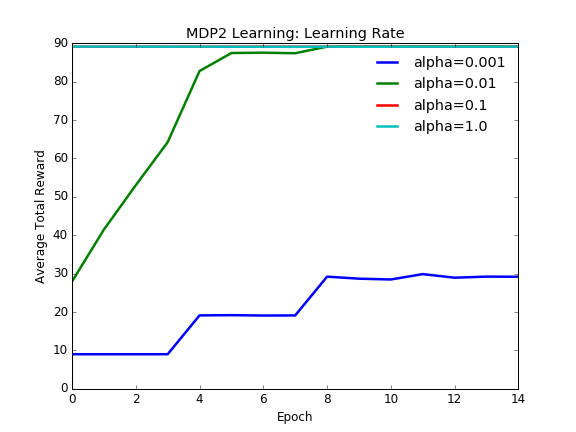
\includegraphics[width=.8\linewidth]{mdp2_alpha_plot.png}
\caption{Plot of average total reward as a function of epochs for different learning rate $\alpha$ values using MDP2 and fixing $\epsilon=0.1$.}
\label{fig:mdp2_alpha}
\end{figure}

\subsection{Discussion}

First, we analyze what changing $\epsilon$ does. For MDP1, we see in Figure \ref{fig:mdp1_epsilon} that for $\epsilon=0.1,0.25,0.5$ the average total reward eventually converges at epoch 14 to the average total reward as reported from using the optimal policy. For $\epsilon=0.75$, the behavior is a bit erratic and would probably converge to the average total reward using the optimal policy had there been more epochs. We also see a similar behavior for MDP2 in Figure \ref{fig:mdp2_epsilon}. The erratic behavior and slow convergence for $\epsilon=0.75$ makes sense since a higher $\epsilon$ means higher probability of exploration constantly.  Higher probability of exploration is good at the beginning when we have no knowledge. However, as we gain more knowledge we should start exploiting it rather than exploring. The experiment confirms that intuition. Overall, the plot is also a good check that the Q-learning reinforcement learning algorithm is indeed learning the optimal policy through Q-tables since the average total reward converges to that of the optimal policy.

Next, we analyze what changing learning rate $\alpha$ does. For MDP1, we see in Figure \ref{fig:mdp1_alpha} that for $\alpha=0.01, 0.1$ the average total reward eventually converges at epoch 14 to the average total reward as reported from using the optimal policy. For $\alpha=0.001$, the average total reward grows slowly and will probably converge to the average total reward using the optimal policy had there been more epochs. For $\alpha=1.0$, the behavior is eratic: it converges at first, but then oscillates to lower values. Overall, the lower the $\alpha$ the more stable the training and the more slowly until convergence. The higher the $\alpha$, the faster the training but a high enough $\alpha$ will cause instability. This makes sense and is consistent with learning algorithms like gradient descent.

For MDP2, the analysis of $\alpha$ is slightly different as shown in Figure \ref{fig:mdp2_alpha}. We see that for $\alpha=0.01, 0.1, 1.0$ the average total reward eventually converges at epoch 14 to the average total reward as reported from using the optimal policy. The difference is that $\alpha=1.0$ is no longer unstable and in fact converges. This probably makes sense for MDP2 since the optimal behavior would be to park at the handicap spots since it has the highest reward. This rule of always choosing the handicap spot seems easier to learn. Finally for $\alpha=0.001$, the average total reward grows slowly and will probably converge to the average total reward using the optimal policy had there been more epochs. This is the same as before.

\section{Code}

Run the code as follows:

\begin{verbatim}
python setup.py
source venv/bin/activate
python main.py
deactivate
\end{verbatim}

The setup script creates a Python virtual environment and main.py runs the script for all parts of the assignment. The setup script is not necessary if numpy is already installed on the system.

\end{document}